
The ATLAS calorimeters are designed to efficiently capture, and
precisely measure, the energy of photons, electrons, and hadrons. They
are symmetric about the beam axis and extend beyond the ID to $|\eta|
= 4.9$~\cite{bib:Aad:2008zzm}. The electromagnetic calorimeter, optimized for electrons and
photons, is segmented into a barrel and two end-caps. Its barrel is
housed in a liquid argon cryostat. The two end-caps have separate
cryostats that also contain the hadronic end-cap calorimeter (HEC) and
the forward calorimeter (FCal). Beyond the barrel EM calorimeter is
the hadronic tile calorimeter. A drawing of entire calorimeter system is
displayed in figure~\ref{chap:detector:fig:calorimeter}.

\begin{figure}[ht]
    \centering
    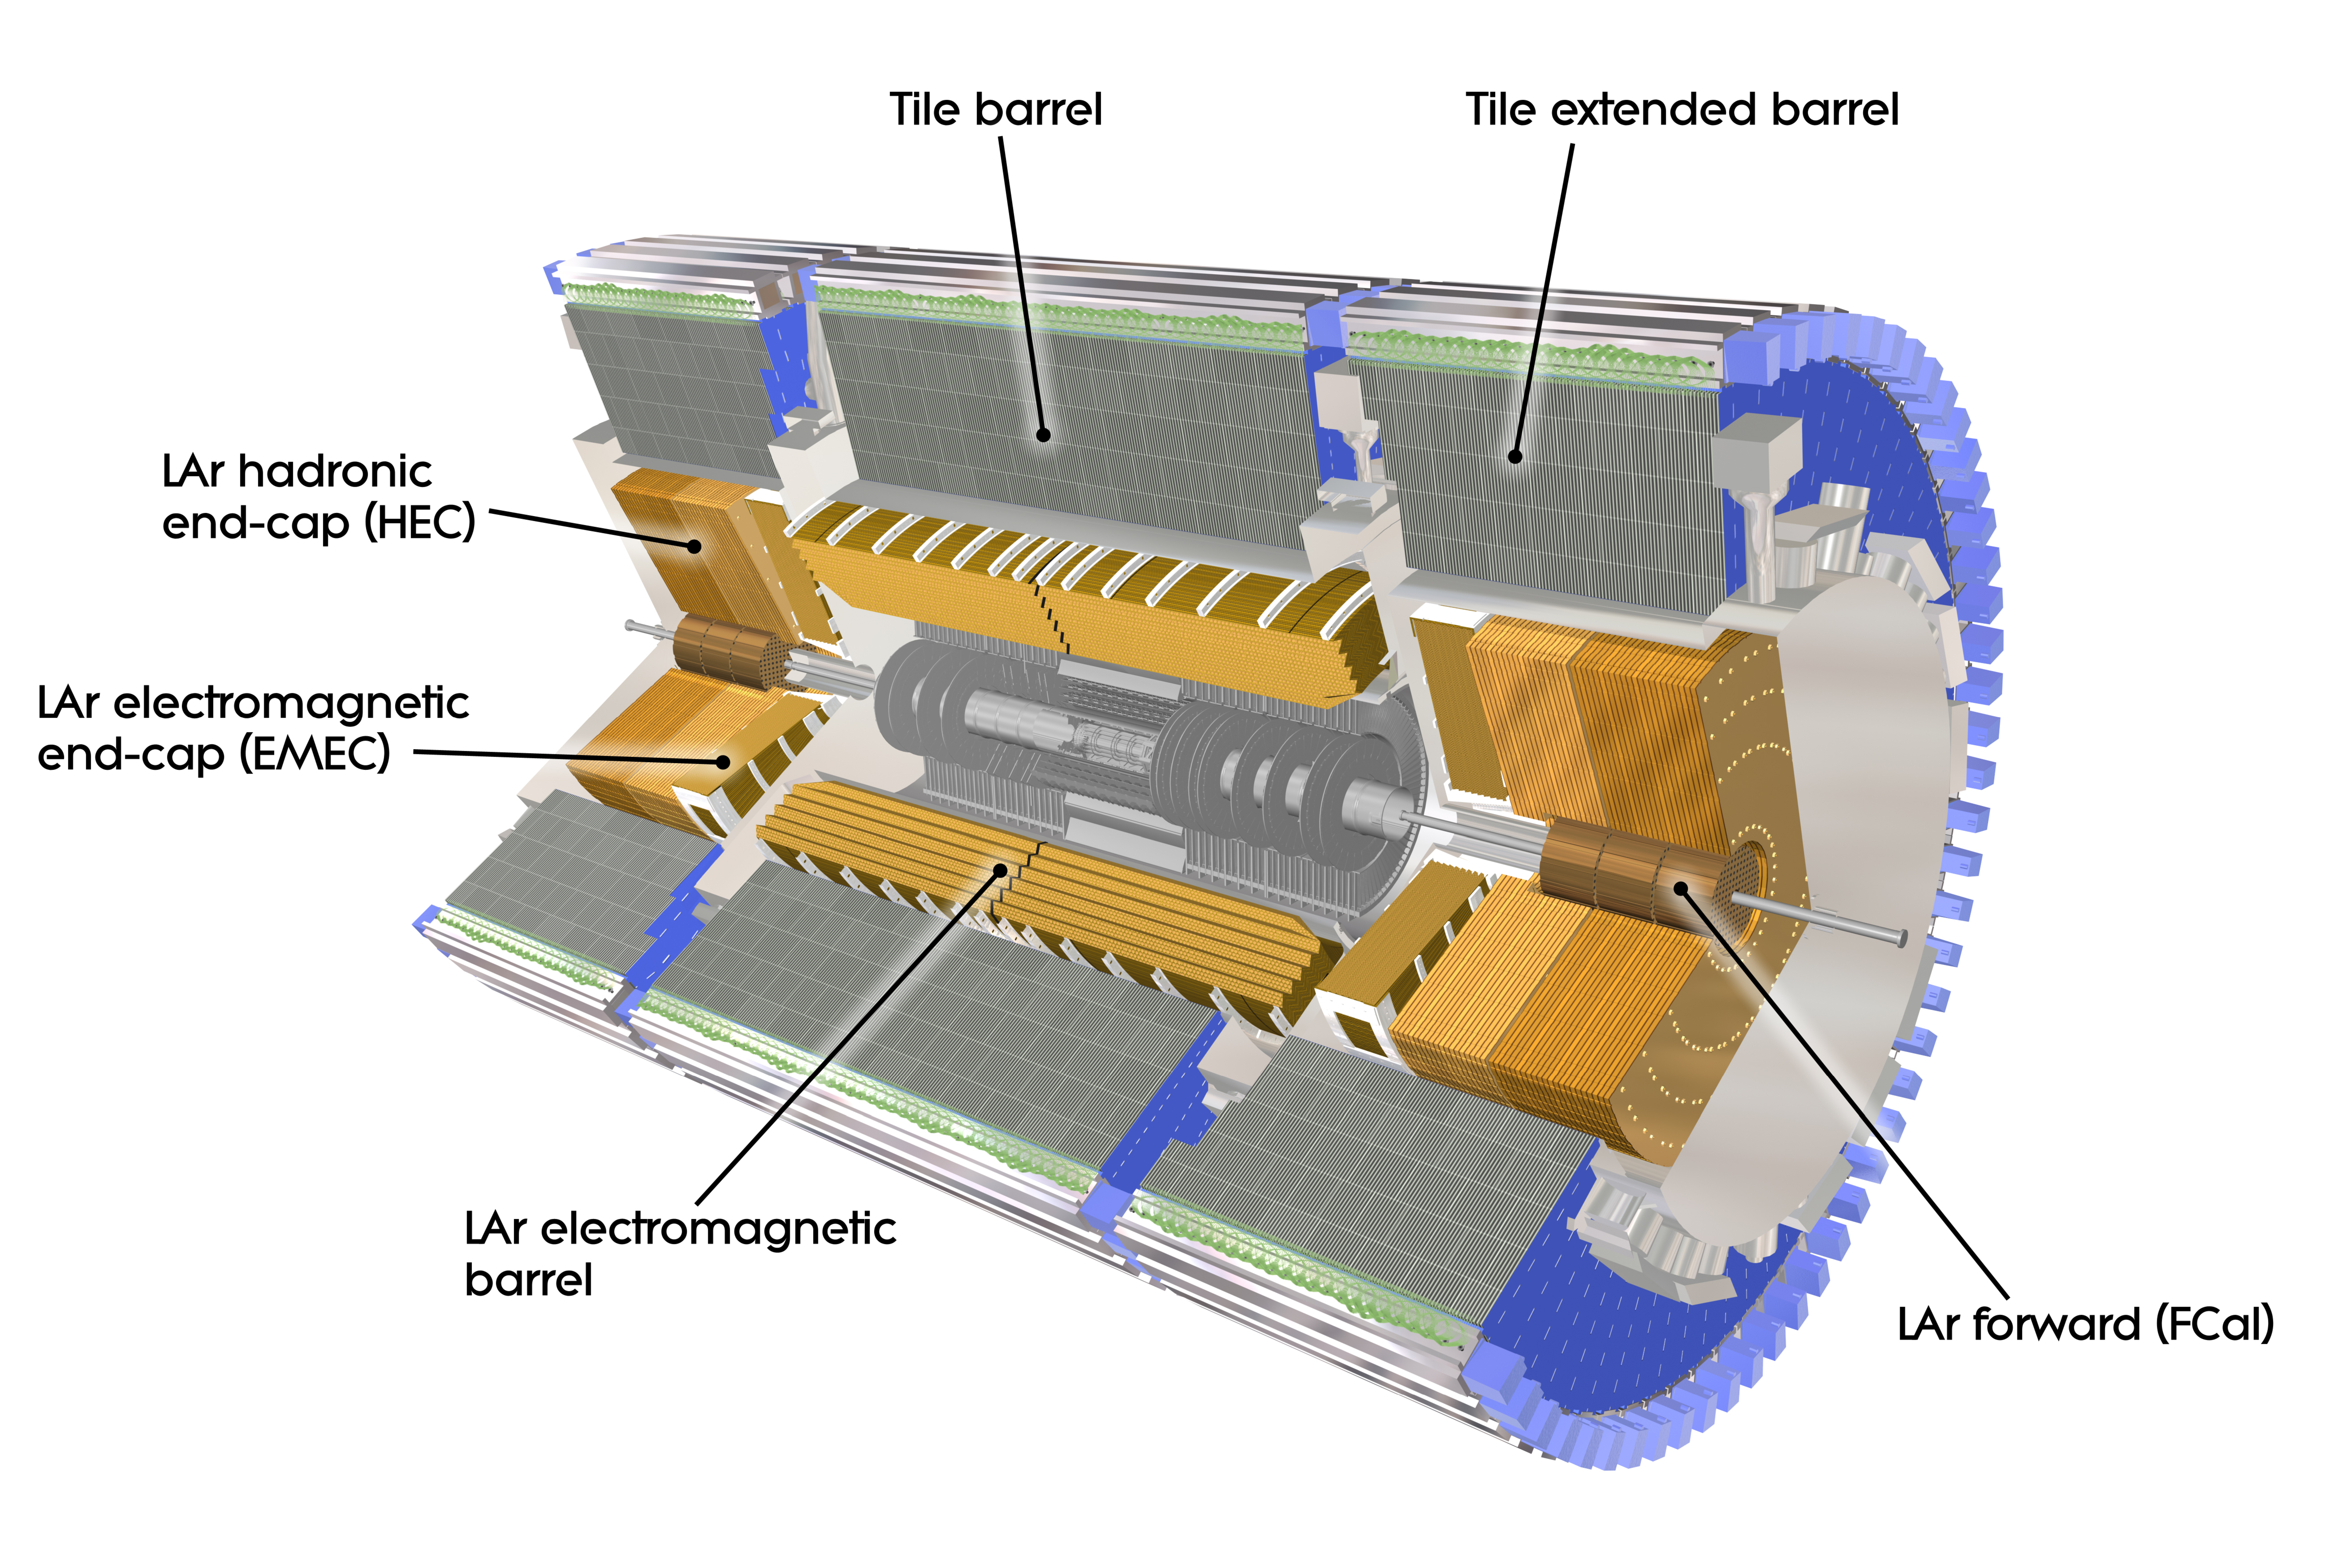
\includegraphics[width=0.8\textwidth]{fig/detector/full_calorimeter.pdf}
    \caption[]{}
\label{chap:detector:fig:calorimeter}
\end{figure}

\subsection{Liquid argon electromagnetic calorimeter}

The barrel of the EM calorimeter spans the region $|\eta|<1.48$, and
is split into two halves at $\eta = 0$. Lead plates with an accordion
geometry provide the needed absorbing material. This geometry, shown
in figure~\ref{chap:detector:fig:accordion}, yields uniform azimuthal coverage and fast detector
response~\cite{bib:Aad:2008zzm}. The readout electrodes are positioned parallel to
the lead plates in the center of the gap between adjacent plates. Each electrode
consists of three layers of copper separated by a thin insulating layer of
polyimide. The outer layers are set to the high voltage potential, and the
inner layer carries the signal to the electronics by
capacitive coupling. These electrodes are etched in order to define
the granularity in the $R$ and $\eta$ directions. The $\phi$
granularity is set by the spacing of the electrodes and how they are
integrated into the front-end electronics~\cite{bib:Aubert:2005dh}. The calorimeter is
subdivided in $R$ into three regions of varying granularity, with the
finest granularity closest to the collision point. In both the $\phi$
and $\eta$ directions, the granularity in the middle layer is 0.025. On either side of
the electrode, the distance is 2.1~mm, corresponding to a drift
time of 250~ns at a nominal voltage of 2.0~kV. The total thickness of
the barrel calorimeter is at least 22 radiation lengths, increasing to 33 as $|\eta|$
increases. 

\begin{figure}[ht]
    \centering
    \includegraphics[width=0.7\textwidth]{fig/detector/em_calo_accordion.pdf}
    \caption[]{\cite{bib:Aad:2008zzm}}
\label{chap:detector:fig:accordion}
\end{figure}

The end-cap segments of the EM calorimeter cover the region
$1.38|\eta|<3.2$, with the overlap ensuring that there is no loss of
resolution in the barrel-end-cap transition region. Each end-cap is
segmented into two concentric wheels, with the inner (outer) wheel composed of
768 (256) lead plates. As for the barrel calorimeter, the plates are
accordion-shaped; however, in the end-cap, the perforations are in the
$R$ direction instead of the $z$ direction. The $R$-$\eta$
segmentation is set by etches in the inter-plate electrodes, forming
three layers of varying granularity, with a granularity of $\Delta\phi
\times \Delta\eta = 0.025 \times 0.025$ in the middle layer. The
thickness of the
end-cap calorimeter varies from 24 to 38 radiation lengths, depending on
$|\eta|$. 

Another important component of the EM calorimeter is the presampler,
located in front of the barrel calorimeter and just outside of the
solenoid coils~\cite{bib:Aad:2008zzm}. Spanning the region $|\eta| < 1.52$, the function of
the presampler is to collect the energy lost by incident particles
before reaching the calorimeter. This correction to the calorimeter
measurement improves the energy resolution by as much as
40\%~\cite{bib:Andrieux:2002xy}. The presampler provides full
azimuthal coverage with 32 modules of width $\Delta\phi = 0.2$ for
each half barrel of the calorimeter. It has a single active liquid
argon layer without any additional absorbing material. To collect
signal, sheets of electrodes are positioned parallel to the
$x$-$y$ plane. Two electrode types--- the anode and cathode--- are
interweaved to achieve a potential difference of 2.0 kV across the
active medium gap of 2~mm. The anode has the same three layer configuration as the
barrel and end-cap calorimeters, allowing the signal to be read out
by the central conductor. Each electrode is etched in the center to
give a $\phi$ granularity of 0.1. The desired $\eta$ granularity is
achieved by electrically connecting adjacent electrodes in the
longitudinal direction, resulting in a constant granularity of 0.025. 

\subsection{Hadronic calorimeters}

Hadrons from the $pp$ collision undergo nuclear interactions in the
detector material. Because these interactions occur at a low rate with
respect to the EM processes that produce energy in the EM calorimeter,
additional calorimeters with greater thickness are positioned beyond
the EM calorimeters. There are three types of hadronic calorimeters:
the barrel tile, the end-cap liquid argon, and the
forward liquid argon. 

The tile calorimeter is segmented into a barrel that covers the region
$|\eta| < 1.0$ and two extended barrels on either side, increasing the
coverage up to $|\eta| = 1.7$~\cite{bib:Abdallah:2008zz}. Each segment
is divided azimuthally into 64 modules. These modules house 4~mm and 5~mm
steel plates, oriented parallel to the $x$-$x$ plane, that act as the
absorbing material (figure~\ref{chap:detector:fig:tile_module}). In the gaps between plates, there are
polystyrene-based scintillating tiles of thickness
3~mm~\cite{bib:Aad:2008zzm}. Ionizing particles
crossing the tiles
produce high frequency visible light that is collected by optical fibers on
either side of the tile. The wavelength of the scintillation light is
shifted by the fibers that also carry the light to
photo-multiplier
tubes (PMTs) on the outer edge of the module, where it is converted to
an electrical signal. By grouping fibers together for
collection into the same PMT, the desired granularity is
obtained. These fiber groups form three layers in the $R$ direction,
with the first two having a granularity of $\Delta\phi
\times \Delta\eta = 0.1 \times 0.1$ and the third with $\Delta\phi
\times \Delta\eta = 0.1 \times 0.2$. The radial depth of the tile
calorimeter is approximately 7.4 nuclear interaction lengths. 

\begin{figure}[ht]
    \centering
    \includegraphics[width=0.5\textwidth]{fig/detector/tile_module.pdf}
    \caption[]{}
\label{chap:detector:fig:tile_module}
\end{figure}

The acceptance of the tile calorimeter is extended by the hadronic
end-cap calorimeter which spans the range $1.5 < |\eta| < 3.2$. Each
end-cap consists of two wheels with the same radius but positioned at
different $z$ values. Both wheels are partitioned in $\phi$ into 32
modules. In the inner (outer) wheel, each module contains 24 (16)
25~mm (50~mm) thick copper plates running parallel to eachother and to the
$x$-$y$ plane. The plates are separated by an 8.5~mm gap that is
further separated into four 1.8~mm liquid-argon-filled drift zones by
three electrodes. The central electrode is a 35 \micron sheet of
copper with 150 \micron of insulating material on each side, while the
outer two electrodes are 75 \micron sheets of polymide between two
insulating layers~\cite{bib:Gingrich:2007ia}. With the two outer
electrodes connected to high voltage, this electrode configuration
forms an electrostatic transformer that equivalent to two 3.6~mm drift
gaps at two times the high voltage of 1800 V. This configuration has
been chosen to minimize ion build up. The detector granularity is
defined by etches in the central copper layer, and in the $|\eta| <
2.5$ ($|\eta| > 2.5$) region, it is $\Delta\phi \times \Delta\eta =
0.1 \times 0.1$ ($0.2 \times 0.2$). 

The last hadronic calorimeter component is the forward calorimeter
(FCal), covering the region $3.1 < |\eta| < 4.9$~\cite{bib:Aad:2008zzm}. Like the
electromagnetic calorimeter and HEC, the ionizing material in the FCal
is liquid argon. Each FCal is segmented into three sub-detectors. The
first (FCal1), which is closest to the IP, is optimized for electromagnetic
showers, and the other two (FCal2 and FCal3) have been designed to contain high energy
hadronic showers. Within the 45~mm FCal1 module are plates of copper
running parallel to the $x$-$y$ plane. A total of 12260 electrodes are
positioned in a 7.5~mm hexagonal array through holes in the plates. Each electrode is a copper
tube coaxial with a copper rod with a gap of 0.269~mm between the
copper surfaces. This small drift length has been chosen to
avoid ion saturation due to high collision
rates~\cite{bib:Artamonov:2008zz}. To ensure near uniformity in the
FCal1 response, the size of the gap between the copper tube and rod is
fixed to within 1\% by an insulating fiber that is wound in a helical
pattern about the copper rod. A potential of 250 V is applied across
the gap (inner rod at high voltage, outer tube at ground), and the
signal is read out by coaxial cables. The signals from groups of
adjacent electrodes are summed in the front-end electronics, forming a
calorimeter cell. Due to the hexagonal geometry of the electrodes, it
is not possible to segment into cells of fixed $\eta$-$\phi$
dimensions. Instead the electrodes are grouped into 16 $\phi$ bins,
each with four $\eta$ bins. 

The FCal2 and FCal3 modules are similar in structure to the FCal1. The
primary difference is that the electrodes are surrounded by tungsten
slugs and the electrode rod is tungsten in order to increase the
absorptivity. Additionally, the spacing of the electrodes is increased
such that the $\eta$ distance spanned by a group of electrodes is
approximately constant across the three FCal modules. The gap spacing
between the electrode rod and tube also increases, to 0.369~mm in
FCal2 and 0.508~mm in FCal3. Finally, just beyond FCal3 is a passive
brass plug to shield the muon system from radiation that has punched
through the FCal. 

